\cotefile{29}
\scanpage{115}
phisme évident
\margin{\figure{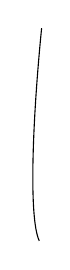
\begin{tikzpicture}\draw (.03,0) .. controls (-.08,-1.1) and (-.14,-2.4) .. (0,-2.7);\end{tikzpicture}}}
\[
\handwritten{\pi}_1^t(U_t)\handwritten{\rightarrow}\handwritten{\pi}_1^t(U)
\]
(un point-base géométrique de $U_t$ étant choisi). Cet homomorphisme est \uline{surjectif}.

Démonstration. Lorsqu'on remplace $L_t$ par $L_{t'}$ générique, alors la conclusion est contenue dans le corollaire 3, en d'autres termes, si $\unsure{\mathbb{U}|\deleted{V}U|\deleted{U}V|\mathbb{V}}$ est un revêtement étale \inserted{connexe} de $U$ \deleted{\unsure{tel que sa,}} (satisfaisant la condition de modération en\deleted{g}visagée - en fait, ce n'est pas nécessaire, enx vertu de 3 ) alors sa restriction $V_{t'}$ au dessus de $U_{t'}$ est connexe. On veut prouver que sa restriction $V_t$ au dessus de $U_t$ est \inserted{\handwritten{également}} connexe. Or pour un paramètre variable sur \inserted{\handwritten{un voisinage ouvert assez petit $T$ de}} la grassmanienne $\deleted{\unsure{T|G}}$ des $L_{t'}$\handwritten{,} \deleted{et voisin de $t$, la famill} \inserted{\handwritten{la}} famille des $Y_{t'}$ est un morphisme propre et lisse $Y\handwritten{\rightarrow}T$, et celle des $D_{t'}$ est un sous-schéma fermé \deleted{de} $\handwritten{\Delta}$ de $Y$, qui est la réunion d'un sous-schéma $\handwritten{\Delta}_1$ qui est de codi\unsure{\deleted{mem}men|\deleted{men}mem}sion $\handwritten{\geq}2$ sur chaque fibre (et qui ne comp\unsure{\deleted{t}|t}e\inserted{\handwritten{\unsure{m|nt|n}}} pas, à cause du théorème de pureté relative) et d'un diviseur $\handwritten{\Delta_2}$ à croise\`{m}ents normaux relatifs. Le revêtement donné $V$ de $U$ définit un revêtement \deleted{$V$ de $Y$} $V'$ de $U'=Y-\handwritten{\Delta}$, et il\deleted{f} faut montrer que la restriction de celui-ci à la fibre géométrique de $t$ est connexe, sachant qu'il en est ainsi de sa restriction à la fibre géométrique en $t'$, la générisation maximale de $t$. Or par la pureté, on sait que $V'$ se prolonge en un revêtement étale $V''$ de $U''=Y-\handwritten{\Delta_2}$, et par hypothèse ce dernier est modérément ramifié sur les fibres, relativement au diviseur $\handwritten{\Delta_2}$. La conclusion est alors une conséquence du théorème \deleted{\unsure{connu}} de spécialisation pour le groupe fondamental modéré, qui figure(ra) dans SGA 1 XIII (exposé de Mme Raynaud).

\uline{Remarque}7.Avec les notations de SGA 7 XVIII\handwritten{,} 6 s'applique pour tout pinceau de Lefschetz $D$ pour fournir la surjectivité de\deleted{s quotients par}
% archive sheet number: 114

\scanpage{116}
l'homomorphisme $\handwritten{\pi}_1^t(D-\overset{\handwritten{\scriptscriptstyle\vee}}{D})\handwritten{\rightarrow}\handwritten{\pi}_1^t(\unsure{\mathbb{P}|\deleted{R}P}-\overset{\handwritten{\scriptscriptstyle\vee}}{X})$, et donne le théorème de conjugaison des cycles évanescents (donc le théorème d'irréductibilité de la cohomologie évanescente) pourvu qu'on ne soit pas dans le cas $\operatorname{car}.k=2$ et $\dim X$ impaire (NB \deleted{ce n'est pas,} dans la situation du th. de Griffiths, il n'y a donc pas d'ennui). Dans ce dernier cas, par contre, je ne sais \deleted{rien} pas prouver\inserted{la conjuga\unsure{\deleted{n}i|i}son sous $\handwritten{\pi}_1(D-\overset{\handwritten{\scriptscriptstyle\vee}}{D})$}, sauf pour un pinceau \uline{générique}, puisqu'alors la représentation envisagée est sauvage; \inserted{j'ignore si \unsure{ella|elle|\deleted{cela}\handwritten{elle}} reste vrai\handwritten{\unsure{e}} pour un pinceau \uline{général}.} Noter cependant que la conjugaison des sous-groupes de monodromie locale\deleted{\unsure{,|s}} \uline{dans} $\operatorname{Aut}(H^{n-1}\handwritten{(Y_{\bar{\eta}}))}$ (qui est très élémentaire) reste vraie, bien entendu, et celle-ci suffit pour prouver le théorème que j'ai proposé (au par. 6 de XVIII) caractérisant le cas où la condition (A) n'est \uline{pas} vérifiée.
% archive sheet number: 115

\scanpage{119}
% archive sheet number: 119

\handwritten{2}. Supposons donné une situation $(Y,V,H,V')$ analogue à $(X,\handwritten{U},G,U')$, et un morphisme $f:X\handwritten{\longrightarrow}Y$ tel que $f(U)\handwritten{\longrightarrow}f(V)$, un morphisme $f':U'\handwritten{\longrightarrow}V'$ compatible avec $U\handwritten{\longrightarrow}V$ induit par $f$, un morphisme de groupes $\handwritten{\phi}:G\handwritten{\longrightarrow}H$ tel que \deleted{$\unsure{f'(gx')=}$} $f'$ soit compatible avec les actions de $G$ et $H$ via $\handwritten{\phi}$, \deleted{et}

Le cas le plus courant sera celui où on se donne un point géométrique $a$ de $U$, \inserted{d'où} un point géométrique $b$ \inserted{$=f(a)$} de $V$, où $U'$ et $V'$ sont respectivement des quotients des revêtements universels de $U$ et $V$ basés en $a$ et $b$, $G$ et $H$ étant respectivement des quotients de $\handwritten{\pi}_{1}(U,a)$ et $\handwritten{\pi}_{1}(V,b)$, l'homomorphisme $f':U'\handwritten{\longrightarrow}V'$ étant induit par les homomorphismes canoniques sur les revêtements universels en $a$ resp. $b$\deleted{\unsure{;|,} \unsure{un tel} $\unsure{f'}$} \unsure{\inserted{\deleted{ainsi que $\handwritten{\phi}$}}} \deleted{\unsure{est} \unsure{donc} déterminé de}, \deleted{façon unique $G$ et $H$ étant les g} $\handwritten{\phi}:G\handwritten{\longrightarrow}H$ étant induit par $f_{\handwritten{*}}:\handwritten{\pi}_{1}(U,a)\handwritten{\longrightarrow}\handwritten{\pi}_{1}(\unsure{\deleted{B}V|\deleted{V}B},b)$ ; de cette façon $f'$ et $\handwritten{\phi}$ sont déterminés sans ambiguïté par $f$, et leur existence signifie simplement que $f_{\handwritten{*}}:\handwritten{\pi}_{1}(U,a)\handwritten{\longrightarrow}\handwritten{\pi}_{1}(V,b)$ veut bien passer au quotient en un $\handwritten{\phi}:G\handwritten{\longrightarrow}H$ (i.e. applique un certain sous-groupe dans un certain sous-groupe). Considérons d'autre part le localisé strict $\handwritten{\overline}{Y}$ de $Y$ en le point géométrique $f(\handwritten{\bar}{x})$ de $Y$, d'où \deleted{\unsure{un}} $\handwritten{\bar}{V},\handwritten{\bar}{V}'$ comme dessus; supposons donné un prolongement $\handwritten{\overline}{Y'}$ de $\handwritten{\bar}{V}'$ en un schéma à groupe d'opérateurs $H$ sur $\handwritten{\bar}{Y}$, et supposons donné enfin un homomorphisme $\handwritten{\overline}{f'}:\handwritten{\overline}{X'}\handwritten{\longrightarrow}\handwritten{\overline}{Y'}$ qui prolonge l'homomorphisme \deleted{\unsure{ft|f'}} $\handwritten{\overline}{U'}\handwritten{\longrightarrow}\handwritten{\overline}{V'}$ induit par $f'$. Pour tout point $\handwritten{\xi}$ de $\handwritten{\overline}{X'}_{\handwritten{\bar}{x}}$, $\handwritten{\overline}{f'}(\handwritten{\xi})$ est alors un point\deleted{s} de $\handwritten{\overline}{Y'}_{\handwritten{\bar}{y}}$, et on peut considérer le groupe d'inertie correspondant $H_{\handwritten{\overline}{f'}(\handwritten{\xi})}$. On a alors la relation évidente
\[
\handwritten{\phi}(G_{\handwritten{\xi}})\handwritten{\subset}H_{\handwritten{\overline}{f'}(\handwritten{\xi})}\ .
\tag*{\handwritten{(2.1)}}
\]
Dans le cas où le\deleted{s} groupe $G$ resp. $H$ opère transitivement sur $\handwritten{\overline}{X'}_{\handwritten{\bar}{x}}$ resp. $\handwritten{\overline}{Y'}_{\handwritten{\overline}{y'}}$, on peut donc dire que $\handwritten{\phi}$ \inserted{applique tout groupe \deleted{de}} \deleted{transforme la classe de conjugaison de sous-groupes} d'inertie de $G$ rel. à $x$ \inserted{\handwritten{\uline{dans}} un groupe d\deleted{e}\handwritten{'}} \deleted{\unsure{en|à} la classe de conj. des sous-groupes} d'inertie de $H$ rel à $y=f(x)$.

\deleted{D'autre part} Il reste alors à expliciter l'homomorphisme $\handwritten{\overline}{f'}:\handwritten{\overline{X'}\longrightarrow\overline{Y'}}$.

\figure{\handwritten{\begin{tikzpicture}[x=0.006cm,y=-0.006cm]
\draw[gray,line width=0.3pt] (1664,451) .. controls (1622,413) and (1571,429) .. (1514,436) .. controls (1119,456) and (709,433) .. (276,428);
\draw[gray,line width=0.3pt] (258,438) .. controls (270,417) and (240,422) .. (228,451) .. controls (206,521) and (206,664) .. (202,870) .. controls (201,912) and (214,941) .. (218,979) .. controls (230,1065) and (230,1149) .. (211,1200) .. controls (236,1219) and (296,1206) .. (347,1208) .. controls (591,1211) and (732,1211) .. (901,1210) .. controls (950,1208) and (976,1188) .. (969,1152) .. controls (1209,1140) and (1415,1155) .. (1601,1137);
\draw[gray,line width=0.3pt,->] (211,1200) .. controls (186,1269) and (152,1426) .. (156,1546) .. controls (153,1742) and (178,1921) .. (203,1996) .. controls (212,2022) and (250,2009) .. (309,2019);
\draw[gray,line width=0.3pt] (63,532) -- (42,549) .. controls (33,559) and (36,583) .. (47,596);
\end{tikzpicture}}}

\scanpage{120}
% archive sheet number: 119

En pratique, il sera vrai que $\handwritten{\overline}{U'}$ est schématiquement dense dans $\handwritten{\overline}{X'}$\inserted{et $\handwritten{\overline}{Y'}$ séparé sur $\handwritten{\bar}{Y}$}, de sorte que $\handwritten{\overline}{f'}$ sera déterminé de façon unique en termes des autres données, comme l'unique prolongement de $\handwritten{\overline}{U'}\handwritten{\longrightarrow}\handwritten{\overline}{V'}$ induit par $f'$; ce sera le cas en particulier dans le cas envisagé plus haut où $\handwritten{\overline}{X'}$ se déduit de \deleted{$\handwritten{\bar}{\unsure{U}}$} $\handwritten{\overline}{U'}$ par normalisation. Bien entendu\deleted{\unsure{r}}, pour pouvoir conclure\inserted{\handwritten{alors}} que tout sous-groupe d'inertie de $G$ rel. à $x$ s'envoie dans un sous-groupe d'inertie de $H$ rel. à $y$, il faudra avoir vérifié l'\uline{existence} d'un p\deleted{p}rolongement $\handwritten{\overline}{f'}$ de $\handwritten{\overline}{U'}\handwritten{\longrightarrow}\handwritten{\overline}{V'}$\inserted{\handwritten{(la commutation aux actions de $G$ dev. alors \uline{automatique})}}. \handwritten{cela \unsure{marchera}, en interprétant $\unsure{\overline{f'}|f'}$ comme $\overline{X'}\unsure{\longrightarrow|-}\overline{Y'}\mathbin{\times}_{\bar Y}\overline{X'}$, lorsque $\overline{Y'}$ est \uline{entier} \deleted{\illegible{1}} sur $\bar Y$, cf. EGA II 6.1.14.}

\handwritten{3.} Revenons à la situation de 1), supposons que $\underline{O}_{X,x}$ soit un anneau local régulier, et que $\handwritten{\bar}{U}$ soit le complémentaire dans le schéma stricte\deleted{\unsure{men}}ment local régulier $\handwritten{\bar}{X}$ d'un diviseur \inserted{$\handwritten{\bar}{D}$} à croisements normaux. On est en particulier dans le cas favorable où la définition de $\handwritten{\overline}{X'}$ est immédiate par normalisation. Supposons que la ramification de $\handwritten{\overline}{U'}$ en les points maximaux de $\handwritten{\bar}{D}$ soit \uline{modérée}. On sait alors, par le calcul local bien connu, que pour tout $\handwritten{\xi\in}\handwritten{\overline}{X'}_{\handwritten{\bar}{x}}$, le groupe d'inertie correspondant $G$ s'identifie canoniquement \deleted{au groupe} à un groupe quotient du groupe
\margin{\handwritten{$C=$ l'ensemble des composantes irred. de $\bar D$}}
\[
I=\handwritten{\prod}_{\handwritten{\unsure{\ell|l}\ne}p}\underline{Z}_{\handwritten{\ell}}(1)(k(\handwritten{\bar}{x}))^C=\handwritten{\prod}_{\handwritten{\ell\ne}p}T_{\handwritten{\ell}}(k(\handwritten{\bar}{x}\unsure{)}\ )^C\ ,
\tag*{(3.1)}
\]
$p$ étant la caractéristique résiduelle en $x$. De p\deleted{\unsure{m}}lus, ce même calc\uline{u}l local montre que le facteur de ce groupe d'inertie correspondant à la composante $\handwritten{\bar}{D}_c$ $(c\handwritten{\in}C)$ du diviseur de ramification $\handwritten{\bar}{D}$ coïncide aussi avec le groupe d'inertie relatif à n'importe quel point de $\handwritten{\overline}{X'}$ au dessus du point maximal de $\handwritten{\bar}{D}_c$ (ou de tout autre point de $\handwritten{\bar}{D}_c$ qui n'appartient à aucune autre composante irréductible de $\handwritten{\bar}{D}$) qui générise $\handwritten{\xi}$ ; comme il y a toujours de tels points, cela montre que la classe de conjugaison du facteur en question peut aussi s'interpréter comme la \deleted{grou} classe des groupes d'inertie en les points envisagés de $\handwritten{\bar}{D}_c$ ; en particulier, cette classe de conjugaison ne dépend que de la composante irréductible de $D=X-U$ \deleted{, image} de point générique l'image du point générique de $\handwritten{\bar}{D}_{\handwritten{c}}$.

\scanpage{121}

\handwritten{4.} Revenons à la situation de 2, et supposons que la structure de $(\handwritten{\bar}{X},\handwritten{\bar}{U})$ soit celle envisagée dans 3, et que de même $\handwritten{\bar}{Y}$ soit un schéma local régulier et $\handwritten{\bar}{V}=\handwritten{\bar}{Y}-\operatorname{supp}\handwritten{\bar}{E}$, $\handwritten{\bar}{E}$ étant un diviseur à croisements normaux sur $\handwritten{\bar}{Y}$. Soit $C'$ l'ensemble des composantes irréductibles de $\handwritten{\bar}{E}$, On voit alors que pour tout $c'\handwritten{\in}C'$, l'image inverse de $\handwritten{\bar}{E}_{c'}$ est un diviseur sur $\handwritten{\bar}{X}$ dont le support est contenu dans celui de $\deleted{\unsure{E}}\handwritten{\bar}{D}$, donc est de la forme
\[
\handwritten{\bar}{f}(\handwritten{\bar}{E}_{c'})=\handwritten{\sum}_{c}\unsure{a|n}_{c,c'}\handwritten{\bar}{D}_c\ ,
\]
où pour $c'$ fixé, les $n_{c,c'}$ sont des entiers $\handwritten{\geq}0$ non tous nuls. Ces notations fixées, un calcul immédiat \deleted{\unsure{direct}} d'images inverses de revêtements kummériens montre que pour deux points correspondants $\handwritten{\xi}$ et $\handwritten{\eta}$, \deleted{l'homom} on a commutativité dans le diagramme
\diagram{\(\handwritten{(4.1)}\qquad\)
\begin{tikzcd}[ampersand replacement=\&,column sep=large,row sep=large]
\&\handwritten{\deleted{\unsure{H_\xi|G_\xi}}}\&G_{\handwritten{\xi}}^{\handwritten{\deleted{\unsure{\xi|x}}}}\handwritten{\arrow}[r,"{\handwritten{\phi}}","{\deleted{\unsure{N|\phi}}}"']\&H_{\handwritten{\eta}}\\
\handwritten{-}\&{}\handwritten{\arrow}[u,gray]\&\handwritten{\prod}_{\handwritten{\unsure{\ell|l}}}\underline{Z}_{\handwritten{\ell}}(1)(\handwritten{\bar}{x})^C\handwritten{\arrow}[u]\handwritten{\arrow}[r,"N"]\&\handwritten{\prod}^{\handwritten{\prime\prime}}_{\handwritten{\ell}}\underline{Z}_{\handwritten{\ell}}(1)(\handwritten{\bar}{y})^{C'}\handwritten{\arrow}[u]
\end{tikzcd}\(\ ,\)}
les flèches \deleted{horizontales}\inserted{verticales} étant les épimorphismes canoniques, et $N$ étant l'homomorphisme défini par la matrice $N=(n_{c,c'}\handwritten{)}_{(c,c')\handwritten{\in}C\mathbin{\times}C'}$, compte tenu que l'homomorphisme $k(\handwritten{\bar}{y})\handwritten{\longrightarrow}k(\handwritten{\bar}{x})$ induit des isomorphismes
\[
\underline{Z}_{\handwritten{\ell}}(1)(\handwritten{\bar}{y})\handwritten{\xrightarrow{\sim}}\underline{Z}_{\handwritten{\ell}}(1)(\handwritten{\bar}{x})\ .
\]
Pour que \inserted{l'homomorphisme} $N$ soit un isomorphisme, il est donc nécessaire et suffisant que \inserted{$\operatorname{card}C=\operatorname{card}C'$ et que} \deleted{det $N$} l'entier ordinaire $\text{dét }N$ soit égal à $\pm p^r$, où $p$ est l'exposant caractéristique de $k(x)$ et $k(y)$; dans ce cas, on conclut donc que les \inserted{sous-}groupes d'inertie de $H$ en $y$ sont les conjugués des images des \inserted{sous-}groupes d'inertie de $G$ en $x$.

\margin{\handwritten{$\bar E=\unsure{Y^{\vee}|\check Y}$}}
5. Supposons en particulier que l'on ait $V=Y-\operatorname{supp}E$, $E$ étant un diviseur \inserted{$\handwritten{\geq}0$} sur $Y$, \deleted{tel que} $U=f^{\handwritten{-1}}(V)$, et que \deleted{pour tout $\unsure{x\handwritten{\in}}f^{\handwritten{-1}}(E)$, posant} les conditions suivantes soient satisfaites:

\inserted{\handwritten{a) Pour $x\in f^{-1}(\operatorname{supp}E)$, $y=f(x)$, $\underline{O}_{X,x}$ et $\underline{O}_{Y,y}$ sont noethériens.}}

\deleted{\unsure{a}}\handwritten{b}) Le diviseur \inserted{\handwritten{$D=$}} $f^{\handwritten{*}}(E)$ est défini, c'est un sous-schéma \uline{régulier} de
% archive sheet number: 120

\scanpage{122}
% archive sheet number: 121

$\mathbb{X}$ \deleted{et}\inserted{\handwritten{(}donc} $X$ est régulier en les points de son support\handwritten{)},\deleted{$U=f^{\handwritten{-1}}(V)\handwritten{\unsure{(}}=X-\operatorname{supp}D\handwritten{\unsure{)}}$}.
\margin{\handwritten{\uline{(Condition de transversalité)}}}

\handwritten{b}) $\operatorname{supp}E$ est irréductible, et il est régulier en les points de $f(\operatorname{supp}D)=\operatorname{supp}E\handwritten{\cap}f(X)$ (donc $Y$ est régulier en ses points).

Alors pour tout $x\handwritten{\in}\operatorname{supp}D$, \deleted{\unsure{l'image des}}\inserted{les} sous-groupes d'inertie de $G$ en $x$ \handwritten{o}nt comme images par $\handwritten{\phi}:G\handwritten{\longrightarrow}H$ des sous-groupes de $H$ qui sont des sous-groupes d'inertie de $H$ relativement au point maximal de $\operatorname{supp}E$. Par suite, pour toute représentation linéaire de $G$ (dans un module $M$ sur quelque anneau) \deleted{\unsure{sur}} qui veut bien se factoriser par une représentation linéaire \uline{de} $H$, les images dans $\operatorname{Aut}(M)$ des \inserted{sous-}groupes d'inertie \deleted{\unsure{dans}} de $G$ relatifs aux divers points de $\operatorname{supp}D$ (ou encore, relatifs aux diverses composantes irréductibles de $\operatorname{supp}D$, cela revient au même en vertu de 3\handwritten{)} sont conjugués dans $\operatorname{Aut}(M)$.

\inserted{\uline{Remords\handwritten{\unsure{:}} au n\textsuperscript{o}}\handwritten{s3,4}.} On peut demander \deleted{\unsure{un}}\handwritten{\unsure{des|du}} résultat\handwritten{\unsure{s}} plus précis, en \deleted{\uline{Application}} considérant pour tout $\handwritten{\xi}$ comme ci-dessus (au dessus d'un point géométrique\inserted{$\handwritten{\bar}{x}$} de $\operatorname{supp}D$) l'homomorphisme correspondant $\underline{Z}_{\handwritten{\unsure{\ell|l}}}(1)(\handwritten{\bar}{x})\handwritten{\longrightarrow}G$ dont l'image est le sous-groupe d'inertie correspondant, et en se demandant comment cet homomorphisme varie avec le choix de $\handwritten{\xi}$ \uline{et de} $\handwritten{\bar}{x}$. \unsure{$\overset{\smile}{\underset{\frown}{\text{Pour}}}$} $\handwritten{\xi}$ variable, la variation se fait évidemment modulo composition avec les automorphismes intérieurs de $G$, \deleted{Pour donner un sens à la question} donc pour $\handwritten{\bar}{x}$ fixé, on trouve une classe de conjugaison d'homomorphismes
\[
\underline{Z}_{\handwritten{\ell}}(1)(\handwritten{\bar}{x})\handwritten{\longrightarrow}G\ .
\]
\deleted{pour}\inserted{\handwritten{Étudions}} \deleted{L}\handwritten{l}a variation de cet homomorphisme\handwritten{,} pour $\handwritten{\bar}{x}$ variable dans une composante \deleted{de $D$}\inserted{$D_i$ \handwritten{de}} l'ensemble des points réguliers de $D$\inserted{à car. $\handwritten{\ne\ell}$}; d'après ce qu'on a vu au n\textsuperscript{o}\deleted{\unsure{2}}\handwritten{3}, on passe d'un tel homomorphisme à un autre en composant avec un quelconque des isomorphismes $\underline{Z}_{\handwritten{\ell}}(1)(\handwritten{\bar}{x})\handwritten{\longrightarrow}\underline{\unsure{\mathbb{Z}|E|Z}}_{\handwritten{\ell}}(1)(\handwritten{\bar}{x}')$ associé à une classe de chemins de $\handwritten{\bar}{x}$ à $\handwritten{\overline}{x'}$. Si cet isomorphe ne dépend pas du choix de cette classe de chemins, i.e. si le\deleted{action du groupe fondamental} faisceau \unsure{l|1}-adique de \handwritten{T}ate $\underline{Z}_{\handwritten{\ell}}(1)$ sur $D(\handwritten{\ell})$ est trivial (ce qui se voit déjà sur la

\figure{\handwritten{\begin{tikzpicture}[x=0.006cm,y=-0.006cm]
\draw (1500,0) .. controls (1380,0) and (1340,24) .. (1200,18) .. controls (1000,12) and (810,8) .. (655,16) .. controls (625,20) and (605,18) .. (565,15);
\draw (553,16) -- (506,11) -- (484,90) .. controls (443,86) and (416,94) .. (377,92) .. controls (310,99) and (260,119) .. (222,119) -- (147,107) -- (16,120);
\draw (16,120) -- (24,116) (16,120) -- (24,124);
\draw (14,120) .. controls (10,174) and (23,234) .. (15,288) .. controls (19,365) and (7,421) .. (13,492) .. controls (10,568) and (17,612) .. (17,663) .. controls (19,728) and (20,790) .. (29,851) .. controls (28,914) and (50,953) .. (40,1011) .. controls (25,1050) and (28,1089) .. (34,1142) -- (39,1186);
\draw[line width=0.3pt] (25,138) .. controls (15,199) and (19,253) .. (22,316) .. controls (30,386) and (12,452) .. (17,502) .. controls (22,587) and (8,621) .. (19,693) .. controls (26,774) and (21,833) .. (34,893) .. controls (42,955) and (48,986) .. (36,1036) .. controls (27,1084) and (36,1134) .. (44,1190);
\end{tikzpicture}}}

\scanpage{123}
% archive sheet number: 122

restriction dudit faisceau au \deleted{corps résiduel} point générique de $D_i$, alors \unsure{\deleted{o}\handwritten{b}|\deleted{o}\handwritten{o}}n peut identifier entre eux tous les groupes $\underline{Z}_{\handwritten{\unsure{\ell|l}}}(1)(\handwritten{\bar}{x})$ envisagés à un même groupe $\underline{\mathbb{Z}}_{\handwritten{\ell}}(1)(D_i)$ (qu'on peut interpréter comme groupe des sections de $\underline{Z}_{\handwritten{\ell}}(1)$ sur $D_i$ ou sur le point générique de $D_i$), et on trouve une classe \inserted{de conjugaison} bien déterminée d\deleted{\unsure{r|e}}'homomorphismes $\underline{Z}_{\handwritten{\ell}}(1)(D_i)\handwritten{\unsure{\mathbin{-}|\longrightarrow}}G$. (On trouve un résultat analogue pour les homomorphismes de produits de groupes $\underline{Z}_{\handwritten{\ell}}(1)$ envisagés dans le n\textsuperscript{o}3). Bien entendu, si $\underline{Z}_{\handwritten{\ell}}(1)$ est trivial sur l'ouvert\inserted{$X_{\handwritten{\ell}}$} des points de $X$ \deleted{Lorsque l'on a un $f:X\unsure{\mathbin{-}|\longrightarrow}Y$ comme au n\textsuperscript{o}\unsure{4|2}} de car. $\handwritten{\ne\ell}$, et si ce dernier est connexe, on peut identifier les groupes $\underline{Z}_{\handwritten{\ell}}(1)(D_i)$ au même groupe \inserted{\handwritten{\unsure{à|2}}} $\underline{Z}_{\handwritten{\ell}}(1)(X_{\handwritten{\ell}})$, \deleted{et on} soit $\underline{Z}_{\handwritten{\ell}}(1)$, et on trouve \deleted{un homomorphisme cano} pour chaque $i$ une\deleted{\unsure{homomo}} classe de conjugaison d'homomorphi\unsure{\deleted{s}m|\deleted{m}s|\deleted{s}n|\deleted{n}s}ens $\underline{Z}_{\handwritten{\ell}}(1)\handwritten{\longrightarrow}G$\handwritten{.} En général, celles-ci \deleted{sont} peuvent être distinctes pour des $i$ distincts, bien entendu. Mais relativement à un\deleted{e} morphisme $f:X\handwritten{\longrightarrow}Y$ comme dans les n\textsuperscript{o}2,\handwritten{4}, la formation des classes\inserted{de conjugaison} \deleted{précédentes} d'homomorphismes\inserted{ci-dessus} a un caractère évident de fonctorialité (qu'il y aurait lieu d'énoncer de façon précise, dans le cadre général du n\textsuperscript{o} 4).

\figure{\handwritten{\begin{tikzpicture}[x=0.65cm,y=0.65cm]
\draw (0,11.5) .. controls (0.2,10.8) and (0,9.6) .. (0.3,9) .. controls (0.4,6) and (0.2,3) .. (0.6,0);
\draw (0.7,-0.05) .. controls (1.8,0.1) and (3,0) .. (5,0) -- (9,0) .. controls (9.4,0) and (9.2,0.4) .. (9.7,0.35) .. controls (11.5,0.1) and (13,0.2) .. (15,0.5);
\end{tikzpicture}}}

Revenant alors aux conditions du présent n\textsuperscript{o}5, on peut préciser de la façon suivante l'assertion faite sur les \deleted{grou} classes de conjugaison de sous-groupes d'inertie en des assertions sur les classes de conjugaisons d'\unsure{\deleted{b}h|\deleted{h}b}\uline{omomorphism}es \uline{de modules de Tate}: supposons que $Y_{\handwritten{\ell}}$ soit connexe et que $Z_{\handwritten{\ell}}(1)$ soit trivia\unsure{\deleted{o}l|\deleted{l}o|\deleted{b}l|\deleted{l}b} sur $Y_{\handwritten{\ell}}$, \deleted{\unsure{d'où|d'on} un isomorphisme désignant} de sorte qu'on peut identifier $Z_{\handwritten{\ell}}(1)(Y_{\handwritten{\ell}})$ et les divers $\underline{Z}_{\handwritten{\ell}}(1)(D_i)$ à un même module \handwritten{(}libre de rang 1\handwritten{)}$\underline{Z}_{\handwritten{\ell}}(1)$ sur $\underline{Z}_{\handwritten{\ell}}$. Considérons alors les classes de conjugaison d'homomorphismes composés
\diagram{\begin{tikzcd}[ampersand replacement=\&,column sep=1.4cm]
\underline{Z}_{\handwritten{\ell}}(1)\handwritten{\arrow}[r,"{\text{inertie en }D_i}"]\&[4.2cm]G\handwritten{\arrow}[r,"{\handwritten{\phi}}"]\&H
\end{tikzcd}\(.\)}

Ces classes sont conjuguées entre elles.

\scanpage{125}
\mspage{\handwritten{\textcircled{1}}}
% archive sheet number: 124

\handwritten{\unsure{Vallouin|Valloire|Vallouise} 18.\unsure{6|8}.1959}\\

Mon cher Serre;\\

Tate m'a écrit de son côté \deleted{pour} sur ses histoires de courbes elliptiques, et pour me demander si j'avais des idées sur une définition globale des variétés \unsure{anglytiques|anplytiques} sur des corps valués complets. Je dois avouer que je n'ai pas du tout compris pourquoi ses résultats suggèreraient l'existence d'une telle définition, et suis encore sceptique. Je n'ai pas non plus l'impression d'avoir rien compris à son théorème, qui \deleted{pour moi} ne fait que exhiber par des formules brutales un certain isomorphisme de groupes analytiques; \deleted{et} on conçoit que d'autres formules tout aussi explicites en donneraient un autre pas plus mauvais (sauf preuve du contraire !)

J'ai réfléchi un petit peu à la partie 'infinitésimale' du groupe fondamental, juste assez pour me convaincre que ça existe et est raisonnable. Voici un contexte (certainement insuffisant d'ailleurs) où ça marche. On a un schéma $S$\inserted{\handwritten{connexe}} (par exemple un schéma algébrique sur un corps $k$), une catégorie auxiliaire $\underline{C}$ (par exemple la catégorie des schémas algébriques finis sur $k$), une catégorie \deleted{de} $\underline{G}$ dont les objets sont des $\underline{C}$-groupes, et les morphismes des morphismes de $\underline{C}$-groupes (par exemple les groupes algébriques finis sur $k$). On \unsure{suppoce|suppose} que dans $\underline{C}$ les produits \deleted{\unsure{finis}}\handwritten{fibrés} existent, et que $\underline{G}$ satisfait aux conditions suivantes: (i) $\underline{\mathbb{G}}$ est stable par produits, et si $u,v:G\handwritten{\longrightarrow}G'$ sont des morphismes dans $\underline{G}$, alors le noyau du couple $(u,v)$ i.e. le sous-groupe \deleted{\illegible{1}} maximum de $G$ où $u,v$ coïncidant -qui existe, car s'exprime par un produit fibré- est dans $\underline{G}$. (ii) Si $u:G\handwritten{\longrightarrow}G'$ est un morphisme dans $\underline{G}$, \deleted{alors il se décompo} le groupe image existe, est isomorphe à un quotient de $G$ comme il se doit, et est dans $\underline{G}$. (iii) Toute suite décroissante de sous-groupes \deleted{\unsure{d'un}} $\handwritten{\in}\underline{G}$ d'un $G\handwritten{\in}\underline{C}$ est stationnaire. On suppose donné de plus un foncteur covariant \deleted{$\unsure{F:\underline{G}|F:\underline{C}}$} $F$ de $\underline{G}$ dans les \deleted{\unsure{G-groupes|S-groupes}} schémas en groupes sur $S$ (par exemple $G\handwritten{\longrightarrow}S\mathbin{\times}_{k}G$), et on suppose : (iv) Le foncteur $F$ commute aux produits, \inserted{\handwritten{aux}} noyaux de coupbes de morphismes, images (on pourra dire que $\unsure{F|\mathbb{F}}$ est ``exact''). (v) Si $H$ est \deleted{un} de la forme $F(G)$ $(G\handwritten{\in}\underline{G})$ alors $H$\inserted{\handwritten{est ``spécial'', i.e.}} admet une suite exacte

\scanpage{127}
\mspage{\handwritten{3}}
\figure{\begin{tikzpicture}[x=0.015cm,y=0.015cm]
\draw[line width=0.4pt] (16,56) .. controls (3,54) and (0,36) .. (8,24) .. controls (17,8) and (44,3) .. (79,13);
\end{tikzpicture}}

De ces deux propriétés résulte formellement qu'on peut trouver un systême projectif \inserted{\handwritten{filtrant}} $(G_i)_{i\handwritten{\in}I}$ dans $\underline{G}$, avec des morphismes $G_i\handwritten{\to}G_j$ qui sont des épimorphismes dans $\unsure{\underline{\mathbb{C}}|\underline{\mathbb{G}}}$, ``essentiellement unique'' dans un sens facile à préciser, tel que \deleted{\unsure{le} foncteur $Z$ soit \unsure{isomorphe}} l'on ait un isomorphisme fonctoriel
\[
Z(G)=\underset{\handwritten{\longrightarrow}}{\lim}\operatorname{Hom}_{\handwritten{\underline{G}}}(G_i,G)
\]

C'est ce systême projectif (pris modulo une équivalence qui intuiti\unsure{v}ment signifie qu'on a passé à la limite projective des $G_i$) qui peut être noté $\handwritten{\pi}^{\underline{G}}_1(S,a)$ et joue le rôle d'un groupe fondamental de $S$ en $a$ (relativement à la catégorìe $\underline{G}$ de groupes, munie du foncteur $F$). Dans le cas \deleted{\unsure{pris}} d'un corps de base $k$, $\underline{G}$ étant la catégorie des groupes algébriques finis sur $k$, on po\uline{urra écrir}e $\handwritten{\pi_1}(S/k,a)$,\margin{\handwritten{à tort}} c'est le groupe proalgébrique (mais avec partie infinitésimale) fondamental du $k$-schéma $S$. Lorsque $k$ est parfait, la décomposition d'un groupe algébrique fini en partie infinitésimale et partie réduite montre que le groupe fondamental est produit semi-direct de sa partie réduite ou séparable \deleted{\unsure{définie}} (qui correspond à un groupe compact discontinu ordinaire\handwritten{,} surlequel le groupe fondamental ordinaire de $k$ - i.e. le groupe de Galois de $\bar{k}$ sur $k$ - opère\inserted{\handwritten{lorsque $a$ est \unsure{rationnel} sur $k$}}), par sa partie infinitésimale, \deleted{\unsure{qui sera un p-groupe fi|qui sera un pro-groupe fi}} qui elle ne dépend d'ailleurs plus du choix du point base $a$ de $S$. Noter que la partie séparable du groupe fondamental peut se réconstituer facilement à l'aide du groupe fondamental ordinaire de $S$ et de son homomorphisme naturel dans $\unsure{\deleted{\mathrm{g}}\mathrm{G}|\deleted{\mathrm{G}}\mathrm{g}}\mathrm{al}(\bar{k}/k)$, \inserted{\handwritten{mais}} il est ``plus grand'' que le groupe fondamental ordinaire, parce\inserted{\handwritten{\,}}qu\deleted{e}\inserted{\handwritten{'}} il correspond à la classification de revêtements principaux de groupe structural non seulement un groupe fini ordinaire, mais un groupe \deleted{\unsure{fini sur lequel}} fini et séparable sur $k$ (i.e. un groupe fini ordinaire sur lequel on fait opérer $\operatorname{Gal}(\bar{k}/k)$ de façon non nécessairement triviale). \deleted{\unsure{Il est}}

J'avoue que si $k$ n'est pas algébriquement clos, le groupe fondamental ci-dessus n'est \deleted{\unsure{peut-être}} \inserted{\handwritten{sans-doute}} pas le bon; on devrait sans doute prendre le groupe fondamental de $S\unsure{\otimes|\times}_{\handwritten{k}}\bar{k}$, qui est un groupe proalgébrique défini sur $\bar{k}$, noter qu'il est muni d'une donnée de descente de $\bar{k}$ à $k$ et est par suite défini en réalité sur $k$; \deleted{avec cette définition, si $S=\operatorname{Spec}(k)$, la \deleted{\unsure{groupe}} partie séparable du groupe fondamental de $S$ (relativement à la ponctuation de $S$ définie par une \deleted{extension \unsure{algé}} clôture algébrique $\bar{k}$ de $k$) n'est autre que}
% archive sheet number: 126

\scanpage{128}
\mspage{\handwritten{4}}
\figure{\handwritten{\begin{tikzpicture}[x=1mm,y=1mm]
\draw[line width=0.4pt] (1.5,5.5) .. controls (0.1,4.6) and (-0.2,2.4) .. (0.6,1.1) .. controls (1.7,-0.2) and (4.7,-0.1) .. (6.4,1.0);
\end{tikzpicture}}}

\deleted{$\operatorname{Gal}(\bar{k}/k)$, mais où en fait opérer $\operatorname{Gal}(\bar{k}/k)$ par automorphismes intérieurs. Ainsi, \deleted{\unsure{les points}} le groupe des points rationnels sur $k$ du groupe fondamental de $\operatorname{Spec}(k)$ s'identifie au centre de $\operatorname{Gal}(\bar{k}/k)$.}

Voici comment on voit l'existence du systême projectif $(\unsure{\mathbb{E}|\mathbb{B}|E}_i)$. Un couple $(\mathbb{G},z)$, avec $G\handwritten{\in}\underline{G}$ et $z\handwritten{\in}Z(G)$, est dit \uline{minimal} si on \inserted{ne} peut trouver un sous-groupe $G'\handwritten{\subset}\underline{G}$ de $G$, \deleted{\unsure{tel que}} $\handwritten{\ne}G$, tel que $z$ soit \deleted{dans} de la forme $Z(i)(z')$, avec $z'\handwritten{\in}Z(G')$ et $i:G'\handwritten{\to}G$ l'injection. \deleted{\unsure{Il}} \handwritten{O}n dit qu'un couple $(G,z)$ est \uline{majoré} par un couple $(G',z')$ si on peut trouver un homomorphisme $\inserted{u:}G'\handwritten{\to}G$ tel que $z=Z(u)(z')$. Il résulte de (iii) que tout couple $(G,z)$ est majoré par un couple minimal, et de la propriété 2) de $Z$ que si $(G',z')$ est minimal et domine $(G,z)$, alors il existe \uline{un seul} $u:G'\handwritten{\to}G$ tel que $z=Z(u)(z')$. De ceci résulte que les couples $(G,z)$ minimaux forment un systême projectif pour la relation de domination, d'ailleurs filtrant (car $(G,z)$ et $(G',z')$ sont dominés par $(GxG',(z,z'))$ lui-même dominé par un $(G'',z'')$ minimal), c'est le systême cherché. On peut si on veut choisir un couple $(G,z)$ dans tout systême de couples \inserted{minimaux} isomorphes, de \deleted{\unsure{qui}} telle façon que l'ensemble d'indices d\deleted{\unsure{onc}} $I$ devient ordonné et non seulement préordonné. (N.B. Ce genre de raisonnements formels est aussi celui qui sert en théorie des \deleted{\unsure{résidus|réseaux}} modules ...).

Je ne sais encore comment devrait être formulée la suite exacte d'homotopie, pour bien faire l'inclusion dans le groupe fondamental d'une partie infinitésimale devrait donner une théorie satisfaisante du comportement du groupe fondamental par spécialisation. J'espère que si $f:X\handwritten{\to}Y$ est un morphisme propre et séparable à fibres absolument connexes i.e. tel que $f(\underline{O}_X)=\underline{O}_Y$, $X$ étant muni \deleted{\unsure{de}} \inserted{\handwritten{pour simplifier}} d'une section \inserted{\handwritten{$s$}} sur $Y$ qui détermine des points-base sur les fibres, alors les groupes fondamentaux \uline{totaux} des fibres de $X$ forment sur $Y$ un \unsure{pro-schéma|proschéma} en groupes \inserted{\handwritten{$\pi_1(X/Y,s)$}} de façon précise qu'on peut trouver un systême projectif \inserted{filtrant} $(G_i)_{i\handwritten{\in}I}$ de schémas en groupes $G_i$ 'spéciaux' sur $\unsure{\deleted{S}Y|\deleted{Y}S}$, avec des homomorphismes $G_i\handwritten{\to}G_j$ qui soient des épimorphismes de $\unsure{\deleted{S}Y|\deleted{Y}S}$-schémas (i.e. correspondant à un homomorphisme injectif de faiscea cohérents sur $\unsure{\deleted{S}Y|\deleted{Y}S}$), de telle façon que les groupes fondamentaux totau\unsure{x} des fibres de $X$ s\unsure{\deleted{r}e|e}\deleted{\unsure{ont}} déduisent dudit pro-schéma en groupes par simple spécialisation. (C'est en tous cas ce que semble indiquer le cas où $X$ est un schéma abélien sur $Y$, cf plus bas).
% archive sheet number: 127

\scanpage{134}
\mspage{I-5}

for $\alpha\handwritten{\ne}o$ the form of the coefficient of $c_\alpha$ implies therefore $\eta_{ij\alpha}=0$ for $i\handwritten{\in}I'$ and $j\handwritten{\in}I''$ since no nonzero linear combination of the $e_j$ is in $W$. Therefore $\xi_{ij}=\eta_{ijo}$ is in $k'$, and $k'$ contains $k(W)$. \hfill q.e.d.

When $V$ is finite dimensional, it follows easily from the previous proof that $k(W)$ is generated by the mutual ratios of the Plücker coordinates of $W$ with respect to any given basis of $V$ rational over $k$.

4.\quad \uline{Rationality for linear and multilinear maps.}

We shall investigate in this paragraph the question of rationality for the multilinear maps. Two particular cases are worth mentioning; the first concerns the linear maps, the second the multilinear and linear forms, that is the case of functions with values in $K$ endowed with the $k$-structure defined by $k$.

Let $V_i$ for $1\leq i\leq r$ and $W$ be vector spaces, each one endowed with a $k$-structure. A multilinear map $f$ from $V_1\times\ldots\times V_r$ to $W$ is called rational over $k$ if $f(v_1,\ldots,v_r)$ is rational over $k$ when the $v_i$ do. It is clear that any multilinear map obtained by composition of some multilinear maps rational over $k$ is rational over $k$.

Let $\{e_\alpha^{(i)}\}$ be a basis of $V_i$ rational over $k$ (for $1\leq i\leq r$); since any vector in $V_i$ rational over $k$ is a linear combination with coefficients in $k$ of the basic elements, a multilinear function $f$ as before is rational over $k$ if and only if $f(e_{\alpha_1}^{(1)},\ldots,e_{\alpha_r}^{(r)})$ is rational over $k$ whatever be the indices $\alpha_1,\ldots,\alpha_r$; if $\{e'_j\}$ is a basis of $W$ rational over $k$ and if one puts
\[
f(e_{\alpha_1}^{(1)},\ldots,e_{\alpha_r}^{(r)}=\sum_j f^j_{\alpha_1,\ldots,\alpha_r}\cdot e'_j
\tag*{(4)}
\]
the function $f$ is rational over $k$ if and only if the components $f^j_{\alpha_1,\ldots,\alpha_r}$ are in $k$. From that follows two facts:

a. Let $k'$ be a field. In order that $f$ be rational over $k'$, it is necessary and sufficient that $k'$ contains the $f^j_{\alpha_1,\ldots,\alpha_r}$, that is the field $k(f)$ generated over $k$ by these elements; in fact, the basis previously introduced are rational over $k$, and \uline{a fortiori} over $k'$.

b. Let us assume the spaces $V_1,\ldots,V_r$ to be finite dimensional. Let $\underline{L}$ be the space of all multilinear maps from $V_1\times\ldots\times V_r$ to $W$, and $\underline{L}_k$ be the

\margin{\handwritten{\unsure{!}}}
% archive sheet number: 133

\scanpage{136}
\mspage{I-4}

$W\handwritten{\cap}V_{k'}=k'\cdot T$ by applying the result a. proved before to $k'$ instead of $k$ and the $k'$-subspace $k'\cdot T$ of $V_{k'}$. Otherwise stated, $W$ is rational over $k'$ and $W\handwritten{\cap}V_{k'}=k'\cdot(W\handwritten{\cap}V_k)$ in such a way that the two $k'$-structures one could get on $W$ by extension of scalars and inducing are actually the same.

We shall now characterize the fields over which a given subspace is rational.

\uline{Proposition} 1.\quad \uline{Let} $V$ \uline{be a vector space with a} $k$-\uline{structure}. \uline{For any subspace} $W$ \uline{of} $V$\unsure{.|:} \uline{there exists a field} $k(W)$ \uline{such that the relations} ``$W$ is \uline{rational over} $k'$'' \uline{and} ``$k(W)$ \uline{is contained in} $k'$'' \uline{are equivalent for any field} $k'$.

Let $\{e_i\}_{i\handwritten{\in}I}$ be a basis of $V$ rational over $k$; by standard results, there is a subset $I''$ of $I$ such that the vectors $e_j$ for $j$ in $I''$ form a basis of $V$ modulo $W$. This means that $V$ is direct sum of $W$ and the subspace $V''$ having $\{e_j\}_{j\handwritten{\in}I''}$ as a basis; but $V$ is direct sum of $V''$ and the subspace $V'$ having as a basis the $e_i$ for $i$ in $I'=I-I''$. Therefore there exists a unique isomorphism $f$ of $V'$ with $W$ such that $f(v')-v'\handwritten{\in}V''$ for any $v'$ in $V'$. If one puts $v_i=f(e_i)$ for $i\handwritten{\in}I'$, the vectors $v_i$ form a basis of $W$ and they are of the following type
\margin{\handwritten{\unsure{!|;}}}
\[
v_i=e_i-\sum_{j\handwritten{\in}I''}\xi_{ij}\cdot e_j\qquad(i\quad I')
\tag*{(2)}
\]
for some scalars $\xi_{ij}$ in $K$ ($i\handwritten{\in}I'$ and $j\handwritten{\in}I''$). Moreover, no non zero linear combination of the $e_j$ for $j\handwritten{\in}I''$ is in $W$ since $W\handwritten{\cap}V''=0$.

Let $k(W)$ be the field generated over $k$ by the $\xi_{ij}$. If a field $k'$ contains $k(W)$, the vectors $v_i$ are rational over $k'$ and so does $W$. Conversely, suppose that $W$ is rational over some field $k'$. Let $\{c_\alpha\}$ be a basis of $K$ over $k'$ such that $c_o=1$ for some index $\alpha=o$; put $\xi_{ij}=\sum\limits_\alpha\eta_{ij\alpha}\cdot c_\alpha$ with some $\eta_{ij\alpha}$ in $k'$; one gets therefore:
\[
v_i=c_o\cdot(e_i-\sum_j\eta_{ijo}\cdot e_j)+\sum_{\alpha\handwritten{\ne}o}c_\alpha\cdot(\sum_j\eta_{ij\alpha}\cdot e_j).
\tag*{(3)}
\]
Since $W$ is rational over $k'$ and the $v_i$ are in $W$, the considerations in a. above show that the coefficient of each $c_\alpha$ in $v_i$ is in $W$ and rational over $k'$;
% archive sheet number: 135

\cotefile{32}
\scanpage{7}
% archive sheet number: 6

4. \uline{Homomorphisme de Gysin}.

Considérons un diagramme commutatif
\noindent(4.1)
\diagram{\begin{tikzcd}[ampersand replacement=\&,column sep=1.1em,row sep=1.5em]
X \handwritten{\arrow[rr,"f"]} \handwritten{\arrow[dr,"p"']} \& \& Y \handwritten{\arrow[dl,"q"]} \\
\& S \&
\end{tikzcd}},
avec $p$ et $q$ compactifiables, \inserted{$p$ plat de prés. finie, \deleted{\unsure{de dim}} $q$ lisse,} $\unsure{\deleted{A}S|\deleted{S}A}$ étant muni d'un Anneau de torsion $A$ premier aux car. résiduelles. Pour un complexe de $A$-modules $F$ sur $S$, on définit alors un homomorphisme canonique
\[
\handwritten{\mathrm{Tr}_f\ \text{ou}\ }f_{\handwritten{*}}:\quad \mathrm{R}f_{\handwritten{!}}(F_X)\handwritten{\longrightarrow} F_Y(d'-d)\handwritten{[}2(d'-d)\handwritten{]},
\tag*{(4.2)}
\]
en supposant $p,q$ de dimensions relatives $d,d'$ en tout point (il suffit que $p$ soit de dim rel $\handwritten{\leqslant} d$ en tout point). Si $p$ est également lisse et de dim. rel. exactement $d$ partout, alors l\unsure{\deleted{h}'|\deleted{'}h}homomorphisme précédent s'identifie à l'homomorphisme d'adjonction pour $\mathrm{R}f_{\handwritten{!}}$, $\mathrm{R}f^{\handwritten{!}}$ relatif au deuxième membre. En tous cas, l'homomorphisme en question s'appelle \uline{homomorphisme de Gysin} (relatif à $f,F$), ou \uline{homomorphisme trace} (\unsure{parfois} noté $\mathrm{Tr}_f$). On \unsure{\deleted{d}a|\deleted{a}d}\unsure{\deleted{a}p|\deleted{p}a}pelle encore par le même nom, et on note de même, tout homomorphisme déduit de (4.2) par application d'un foncteur quelconque (le \deleted{cas échéant}\inserted{\handwritten{plus souvent,}} en transformant encore la flèche obtenue en appliquant des isomorphismes canoniques, tels des isomorphismes de transitivité ... , utilisés communément \deleted{\unsure{à d}} comme morphismes d'identification ...), Par exemple on a les homomorphismes
\[
\mathrm{H}^i(f_*)\ \text{ou}\ f_*:\quad \mathbb{R}^i f_{\handwritten{!}}(F_X)\handwritten{\longrightarrow} \underline{\unsure{\mathbb{H}|\mathrm{H}}}^{i\inserted{\handwritten{+2(d'-d)}}}_{\deleted{\unsure{Y|*}}}(F_{\inserted{\handwritten{Y}}})_{\deleted{\unsure{Y|*}}}(d'-d)\deleted{\unsure{[2(d'-d)}},
\tag*{(4.2.1)}
\]
de faisceaux sur $Y$, déduit\handwritten{s} de (4.2?1) en appliquant $\underline{\mathrm{H}}^i$, ou
\[
\mathrm{R}q_{\handwritten{!}}(f_{\handwritten{*}})\ \text{ou}\ f_{\handwritten{*}}:\quad \mathrm{R}p_{\handwritten{!}}(F_X)\handwritten{\longrightarrow}\mathrm{R}q_{\handwritten{!}}(F_Y)(d'-d)\handwritten{[}2(d'-d)\handwritten{]},
\tag*{(4.2.2)}
\]
déduit de (4.2) en appliquant $\mathrm{R}q_{\handwritten{!}}$, ou plus généralement, pour tout morphisme com\unsure{\deleted{â}p|\deleted{p}â}actifiable
\[
g:\ Y\handwritten{\longrightarrow}Z
\]

\scanpage{8}
% archive sheet number: 7
\[
\mathrm{R}\handwritten{(}gf_{\deleted{\unsure{!|*}}}\handwritten{)}_{\handwritten{!}}(F_X)\handwritten{\longrightarrow}\mathrm{R}g_{\handwritten{!}}(F_Y)(d'-d)\handwritten{[}2(d'-d)\handwritten{]}\deleted{\unsure{,|.}},
\tag*{(4.2.3)}
\]
déduit de (4.2) en appliquant $\mathrm{R}g_{\handwritten{!}}$. De même, appliquant $\mathrm{R}g_*$, on trouve
\[
\mathrm{R}g_*\mathrm{R}f_{\handwritten{!}}(F_X)\overset{\mathrm{dfn}}{=}\mathrm{R}(gf)_{\deleted{\unsure{!}}c(f)}(F_X)\handwritten{\longrightarrow}\mathrm{R}g_{\handwritten{*}}(F_Y)(d'-d)\handwritten{[}2(d'-d)\handwritten{\unsure{]} }
\tag*{(4.2.4)}
\]
(où la \deleted{premier}\inserted{source} est ``l'image directe à supports propres sur $Y^{\deleted{\unsure{*}}}$'' )\deleted{\unsure{, qui}}

\deleted{Prenant en particulier} Pour définir cette dernière flèche, \deleted{il était}\inserted{quitte à faire rentrer le $(d'-d)$ dans la parenthèse, il} suffisait de disposer d'un morphisme de \deleted{sites} topos $Y_{\text{ét}}\handwritten{\longrightarrow}Z$, et prenant alors pour $Z$ le topos final, on trouve l'exemple important d'homomorphisme de Gysin:
\[
\mathrm{R}\handwritten{\Gamma}_X(\mathrm{R}f_{\handwritten{!}}(F_X))\overset{\mathrm{dfn}}{=}\mathrm{R}\handwritten{\Gamma}_{X,\deleted{\unsure{!}}c(f)}(F_X)\handwritten{\longrightarrow}\mathrm{R}\handwritten{\Gamma}_Y(F_Y(d'-d))\handwritten{[}2(d'\unsure{\mathord{\perp}|-}d)\handwritten{\unsure{]} }
\tag*{(4.2.5)}
\]
Dans le cas où $f$ est \uline{propre}, (4.2) devient
\[
\mathrm{R}f_{\handwritten{*}}(F_X)\handwritten{\longrightarrow}\mathbb{F}_Y(d'-d)\handwritten{[}2(d'-d)\handwritten{]},
\tag*{(4.2.\unsure{6|5})}
\]
et (4.2.4) et (4.2.5) s'écrivent respectivement
\[
\mathrm{R}(gf)_*(F_X)\handwritten{\longrightarrow}\mathrm{R}g_{\handwritten{*}}(F_Y)(d'-d)\handwritten{[}2(d'-d)\handwritten{]},
\tag*{(4.2.7)}
\]
\[
\mathrm{R}\handwritten{\Gamma}_X(F_X)\handwritten{\unsure{\text{---}|\longrightarrow}}\mathrm{R}\Gamma_Y(F_Y(d'-d))\handwritten{[}2(d'-d)\handwritten{]}.
\tag*{(4.2.8)}
\]

\deleted{Dans (4.2.5) ou (4.2.8), il y aurait lieu de remplacer $F_X$ par un $F_X(i)$} On a également à définir des homomorphismes de Gysin pour des coéfficients sur $Y$ plus généraux que ceux de la forme $F_Y$ et ceux qu'on en déduit par twist et shift. De façon générale, soit $G$\unsure{.|:|;} un complexe de $A$-Modules (NB je ne précise pas ici\inserted{ni ailleurs} les hypothèses de degré) sur $Y$, et appliquons à (4.2) le foncteur $\overset{\mathrm{L}}{\otimes}G$, on trouve un homomorphisme canonique, qui est d'ailleurs le même que si on partait de \deleted{F} $F'=A_S$ sur $S$, et qu'on tensorise l'homomorphisme de Gysin correspendant par $F_Y\otimes G$. Donc, autant oublier $F$ et dire que pour tout $G$ sur $Y$, on a un homomorphisme canonique (dit\inserted{\handwritten{encore}} \uline{de Gysin})
\margin{\handwritten{\fbox{\parbox{1.8cm}{Question: a-t-on besoin d'un $A$ sur $S$, \unsure{ou|ne} suffit d'avoir un Anneau $A_Y$ sur $Y$, de torsion, premier à $Y$ ?}}}}
\[
\boxed{\mathrm{R}f_{\handwritten{!}}(f^{\handwritten{*}}(G))\handwritten{\longrightarrow}G(d'-d)\handwritten{[}2(d'-d)\handwritten{]}},
\tag*{(4.3)}
\]
ou, au choix
